\subsection{Common Setup}
  We propose three different kinds of games, all of them finite (but possibly generalizable to the infinite setting). The first
  consists of one sole strategy where the players do not initially know whether they will be buyers, sellers or nothing at all,
  this being decided in the last moment. The second game consists of three strategies: buyers, sellers and middlemen. The last
  game consists of two strategies: creators and consumers. Before delving into the details of each game, we first describe their
  common elements.
  
  The general approach taken is as follows: After a game is described in detail, each player is assigned a specific strategy and
  a relevant utility function. All players are considered to follow their respective strategy without deviating from it, except
  for one player that is allowed to follow any desired strategy; her utility function however remains unchanged. If that player
  is proven to have an incentive to deviate from her appointed strategy, we can deduce that the given strategies and utility
  functions do not constitute a Nash equilibrium. If on the other hand we can repeat the aforementioned process (keeping all
  players except for one honest) for all given strategies and no player has an incetive to deviate, then we will come to the
  conclusion that the given strategies and utility functions do constitute a Nash equilibrium. This approach is common in game
  theoretic analyses, given that allowing for all players to be rational and then searching for a Nash equilibrium constitutes a
  practically intractable problem [daskalakis citation]. Another common approach employed is that of considering only a
  generic product that all buyers want and all sellers have, and not a variety of different products.

  A description of the structure that is common for all three games follows. The game graph has a random initial configuration
  where every player has a random direct trust towards every other player, as well as a random capital. These values may be
  uniformly distributed in an interval or may follow another distribution such as the exponential, or may have a high
  probability of being zero. The exact distribution however is not determined at this point, as it is not yet needed. Further
  constraints may be applied to each game separately. This distribution will be common knowledge to the players. Transaction
  fees are not considered.
  
  The players play simultaneously in each round and can do any of the known actions. If two actions conflict (e.g. $A$ reduces
  $DTr_{A \rightarrow B}$ and $B$ steals from $DTr_{A \rightarrow B}$ as well), then one of the two actions is chosen with equal
  probability ($50\%$). To better model a player's actions and the aforementioned conflict resolution, we demand that each
  change explicitly mentions the source and the destination of the funds for each of her actions. Player $A$ decides on the
  values of all the following variables. This constitutes a concrete round for $A$.
  
  \begin{gather*}
    \forall B, C \in \mathcal{V}, move\left(A, \left(A, B\right), \left(A, C\right) \right) = \: ? \\
    \forall B, C \in \mathcal{V}, B \neq A, move\left(A, \left(B, A\right), \left(A, C\right) \right) = \: ?
  \end{gather*}
  The first argument is the player who decides, the second argument is from which direct trust to take the funds and the third
  is to which direct trust to deposit the funds.
  
  To clarify a detail, for any $B \in \mathcal{V}$ (including $A$), $A$ is not allowed to set $move\left(A, \left(A, B\right),
  \left(A, B\right) \right)$ to any value different than 0. This choice is made to facilitate the analysis and because in the
  real-world setting this kind of behaviour has a totally different result, effectively dragging $B$ into an arms race for the
  higher fee. In the real world case, the exact same reasoning goes for $move\left(A, \left(B, A\right), \left(B, A\right)
  \right)$. In our case however, the latter move is already not permitted.
  
  Of course there are some constraints for player's $A$ move:
  
  \begin{itemize}
    \item It makes no sense to deposit to and withdraw from a specific direct trust in the same round. Furthermore, such a
    possibility would allow for "chain reactions" in the conflict resolution phase that would add unnecessary complications.
    This constraint applies only to outgoing direct trusts, because incoming direct trusts cannot be increased.
    \begin{gather*}
      \forall B, C, D \in \mathcal{V}, move\left(A, \left(A, B\right), \left(A, C\right) \right) \times move\left(A, \left(A,
      D\right), \left(A, B\right) \right) = 0 \\
      \wedge \\
      \forall B, C, D \in \mathcal{V}, move\left(A, \left(A, B\right), \left(A, C\right) \right) \times move\left(A, \left(D,
      A\right), \left(A, B\right) \right) = 0
    \end{gather*}
  
    \item One cannot use more funds than are available from a single direct trust.
    \begin{gather*}
      \forall B \in \mathcal{V}, \sum\limits_{C \in \mathcal{V}} move\left(A, \left(A, B\right), \left(A, C\right) \right)
        \leq DTr_{A \rightarrow B} \\
      \forall B \in \mathcal{V}, \sum\limits_{C \in \mathcal{V}} move\left(A, \left(B, A\right), \left(A, C\right) \right)
        \leq DTr_{B \rightarrow A} \\
    \end{gather*}
  \end{itemize}
  
  If two players try to change the same direct trust, then set the relevant moves of one of the two players (chosen uniformly
  at random) to 0.
  \begin{lstlisting}[label=conflict, style=numbers]
resolveConflict((*@$A$@*), (*@$B$@*)) :
  sum1 = (*@$\sum\limits_{C \in \mathcal{V}}move\left(A, \left(A, B\right), \left(A, C\right) \right)$@*)
  sum2 = (*@$\sum\limits_{C \in \mathcal{V}}move\left(B, \left(A, B\right), \left(B, C\right) \right)$@*)
  if (sum1*sum2 != 0)
    choice (*@$ \overset{\$}{\gets} \{A, B\}$@*)
    if (choice == (*@$A$@*))
      (*@$\forall C \in \mathcal{V}, move\left(A, \left(A, B\right), \left(A, C\right) \right)$@*) = 0
    else # if (choice == (*@$B$@*))
      (*@$\forall C \in \mathcal{V}, move\left(B, \left(A, B\right), \left(B, C\right) \right)$@*) = 0

resolveAllConflicts() :
  (*@$\forall A, B \in \mathcal{V}$@*)
    resolveConflict((*@$A$@*), (*@$B$@*))
    resolveConflict((*@$B$@*), (*@$A$@*))
  \end{lstlisting}

  \noindent \texttt{resolveAllConflicts()} is executed after all players choose their moves for a round.

  \begin{figure}[h]
  \label{fig:game}
    \centering
    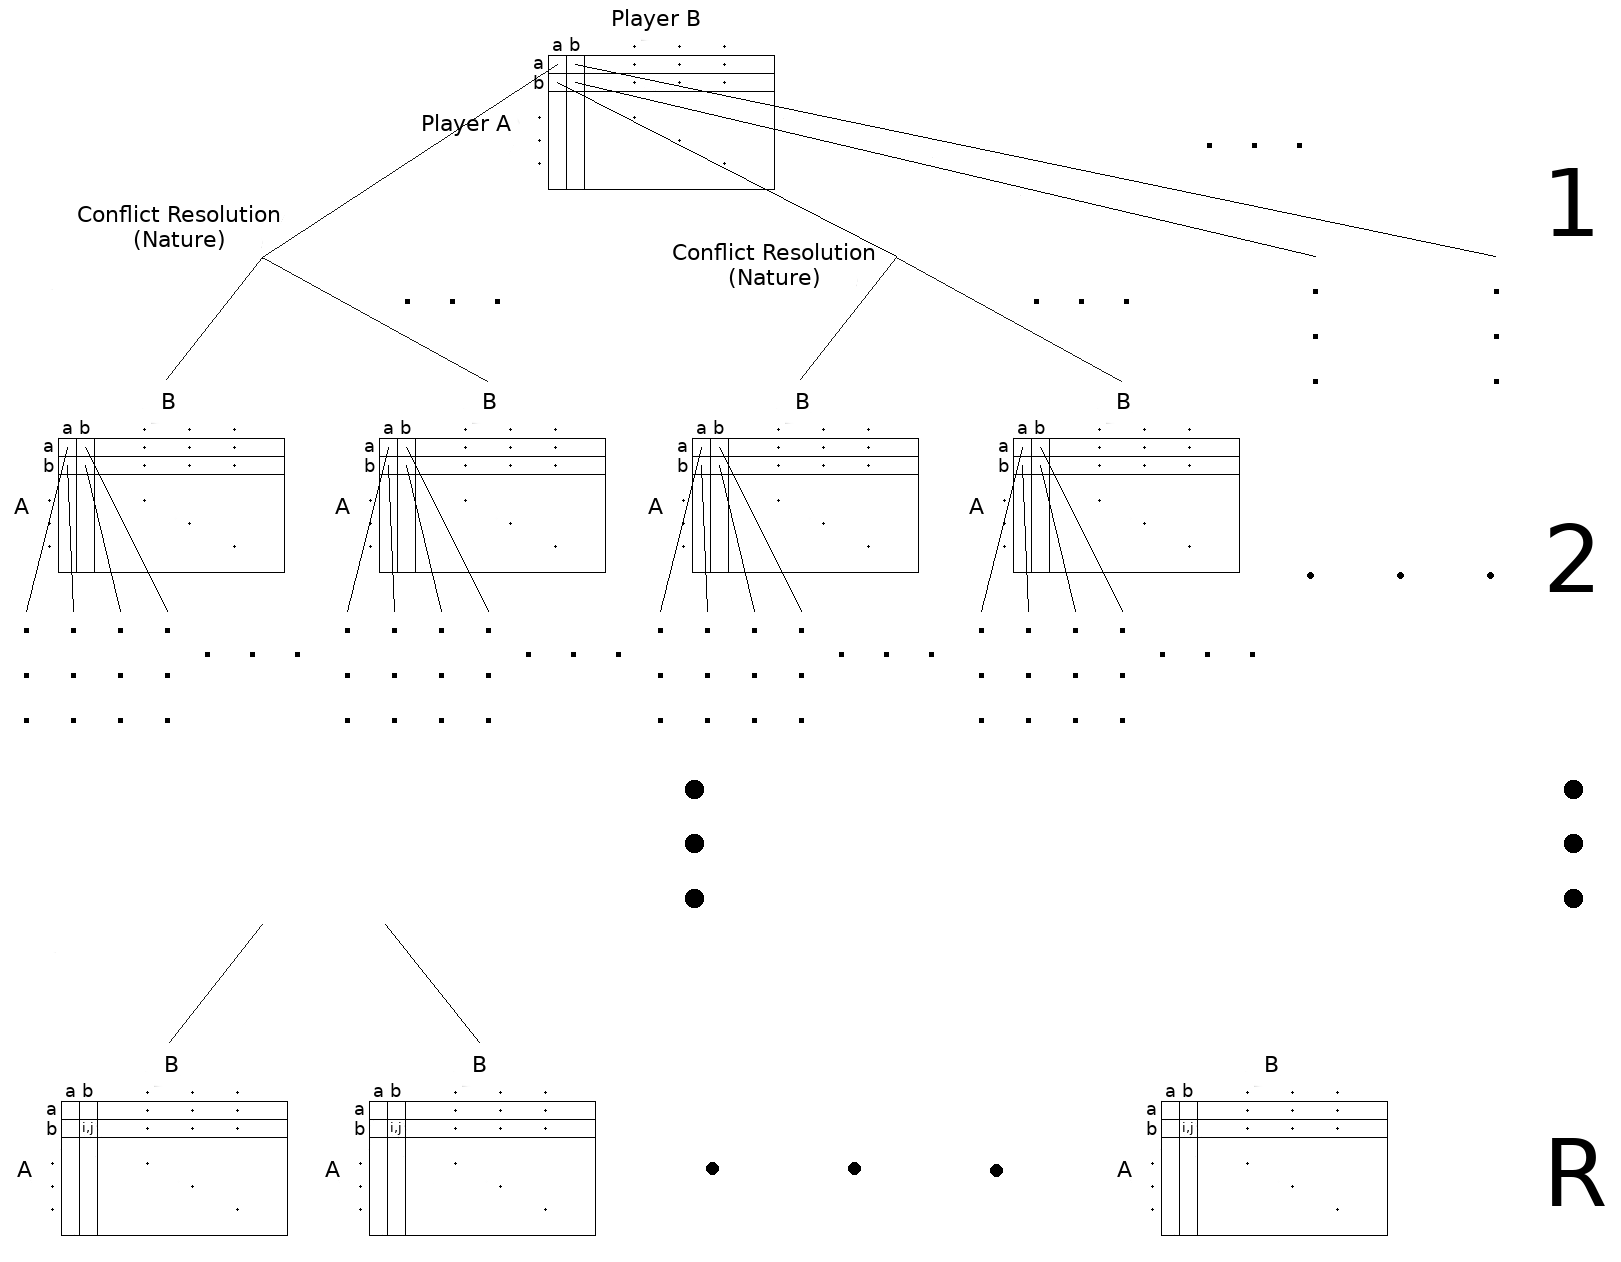
\includegraphics[width=\textwidth]{game}
    \caption{The general form of the game (inspiration due
    \href{http://www.agsm.edu.au/bobm/teaching/SGTM/lect06pr-3.pdf}{here}, p. 3.)}
  \end{figure}
  
  \noindent We now move on to describe the individual games.
